\documentclass[tikz]{standalone}
\usepackage{amsmath}
\usetikzlibrary{arrows.meta,
                bending,
                calc, chains,
                quotes,
                positioning,
                shapes.geometric,
                decorations.pathreplacing,
                calligraphy,
                automata}

\definecolor{pantone2727}{RGB}{48,127,226}

\begin{document}

    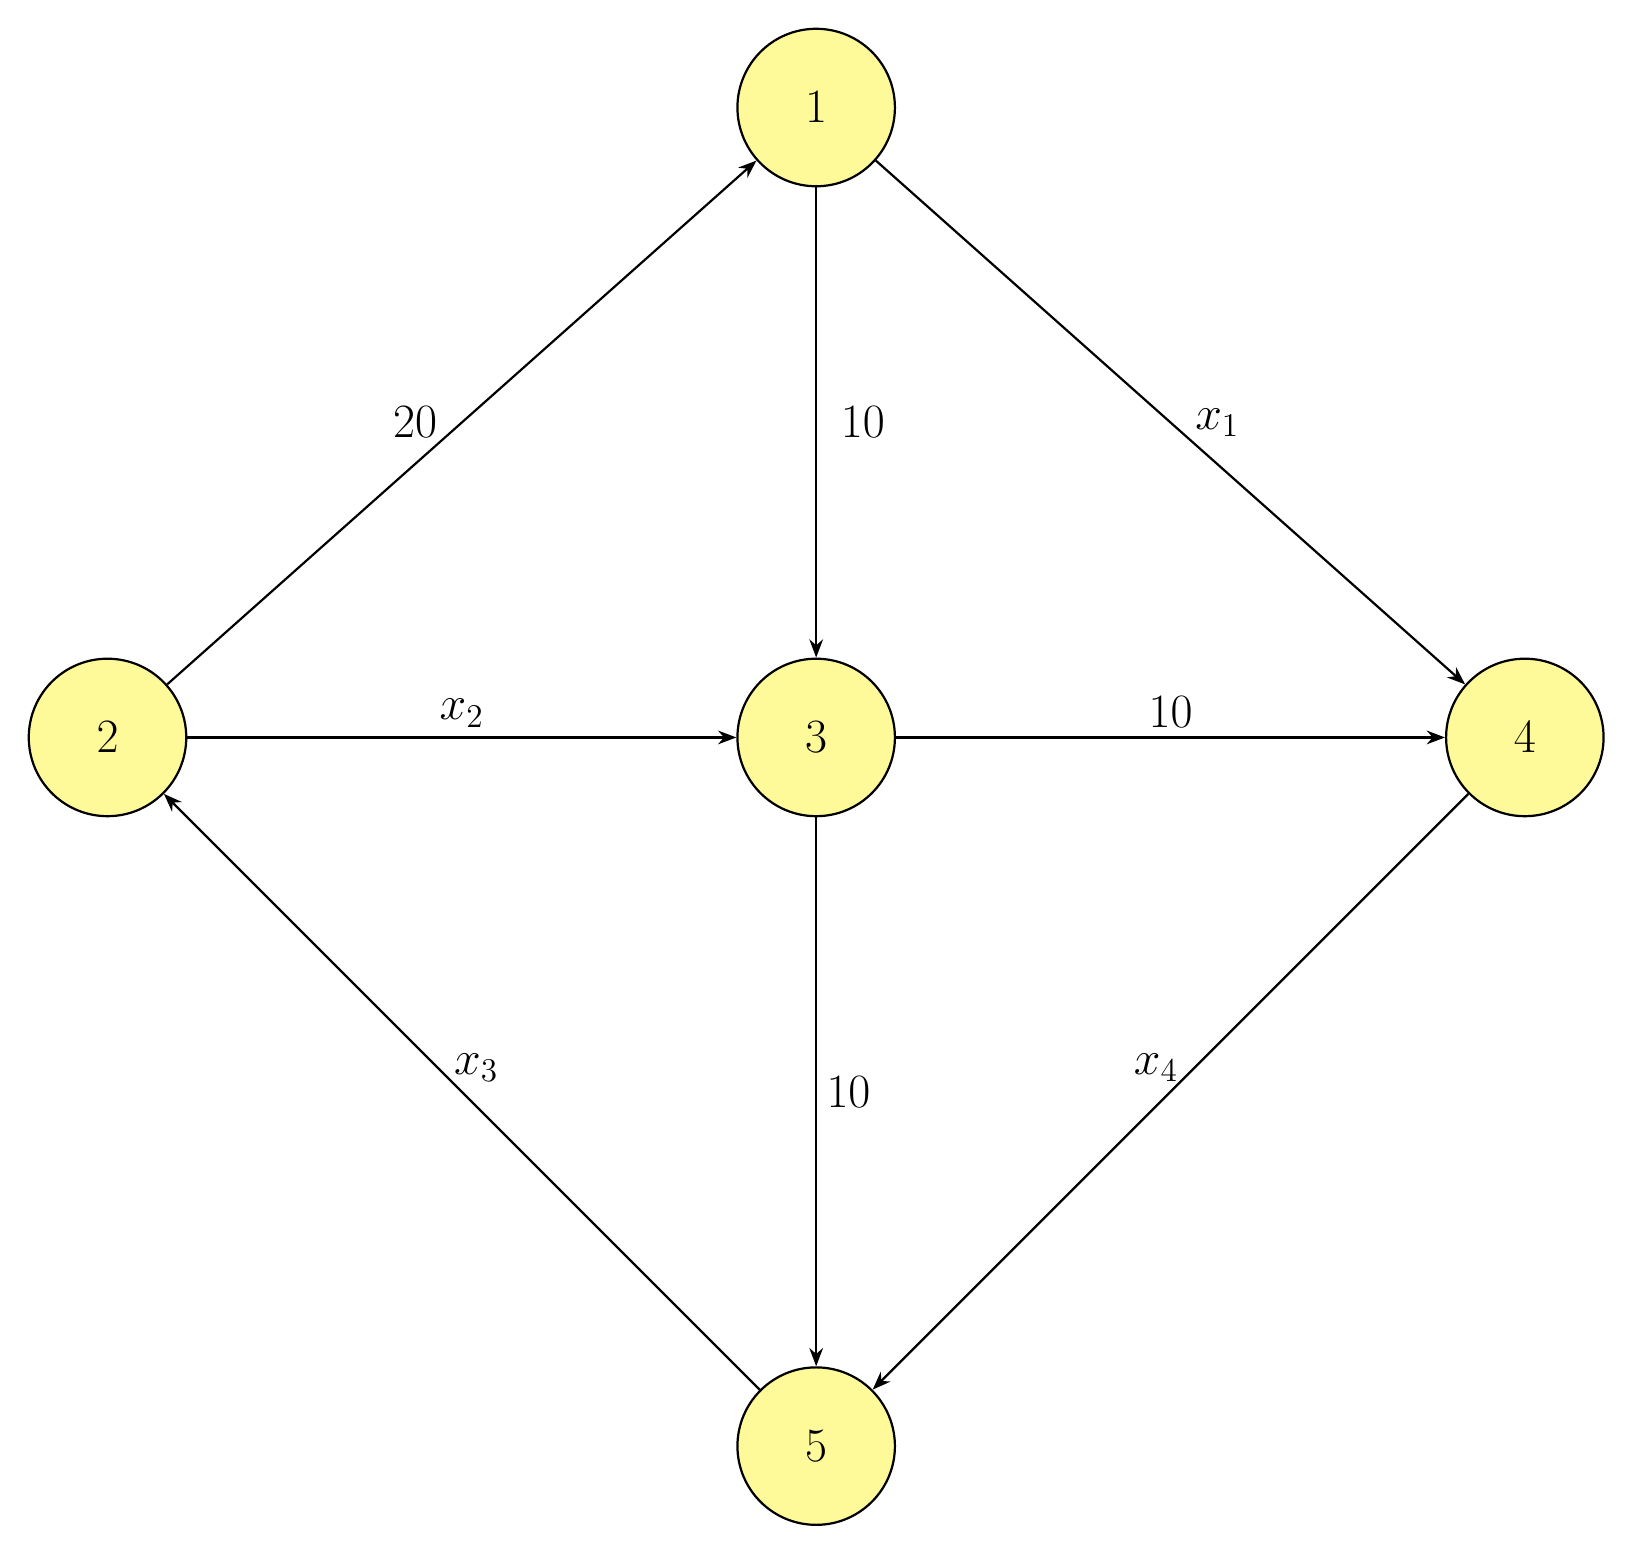
\begin{tikzpicture}[
        node distance=2cm,
        startstop/.style={rectangle, rounded corners, minimum width=3cm, minimum height=1cm,text centered, draw=black, fill=red!30},
        process/.style={rectangle, minimum width=3cm, minimum height=1cm, text centered, draw=black, fill=orange!30},
        io/.style={trapezium, trapezium left angle=70, trapezium right angle=110, minimum width=3cm, minimum height=1cm, text centered, draw=black, fill=blue!30},
        decision/.style={diamond, minimum width=3cm, minimum height=1cm, text centered, text width=3cm, draw=black, fill=green!30},
        end/.style={rectangle, minimum width=3cm, minimum height=1cm, text centered, rounded corners, draw=black, fill=green!30},
        connector/.style={circle, minimum size=2cm, text centered, draw=black, thick, fill=yellow!40}
        ]

        \node (node1)  [connector]                                            {\LARGE 1};
        \node (node2)  [connector, below of=node1, xshift=-9cm, yshift=-6cm]  {\LARGE 2};
        \node (node4)  [connector, below of=node1, xshift=9cm, yshift=-6cm]   {\LARGE 4};
        \node (node3)  [connector, below of=node1, yshift=-6cm]               {\LARGE 3};
        \node (node5)  [connector, below of=node1, yshift=-15cm]              {\LARGE 5};

        \draw [arrows=-Stealth, thick] (node1) -- node[anchor=south]   [right]    {\LARGE $\ x_1$}   (node4);
        \draw [arrows=-Stealth, thick] (node1) -- node[anchor=east]    [right]    {\LARGE $\ 10$}   (node3);
        \draw [arrows=-Stealth, thick] (node2) -- node[anchor=north]   [left]     {\LARGE $20\ $}    (node1);
        \draw [arrows=-Stealth, thick] (node2) -- node[anchor=east]    [above]    {\LARGE $x_2$}     (node3);
        \draw [arrows=-Stealth, thick] (node3) -- node[anchor=east]    [above]    {\LARGE $10$}      (node4);
        \draw [arrows=-Stealth, thick] (node3) -- node[anchor=south]   [right]    {\LARGE $10$}      (node5);
        \draw [arrows=-Stealth, thick] (node4) -- node[anchor=south]   [above]    {\LARGE $x_4\ \ $} (node5);
        \draw [arrows=-Stealth, thick] (node5) -- node[anchor=west]    [above]    {\LARGE $\ \ x_3$} (node2);

    \end{tikzpicture}


\end{document} 